\chapter{Autoregressive Model}
\label{AR}
The Autoregressive Model(AR) is a model for time series analysis. The model specifies that the output variable depends 
linearly on its own previous values and on a stochastic term. An autoregression model of order p can be written as:
\begin{equation}
    y_{t}=\mu_{0}+\epsilon_t \sum^{p}_{i=1}\alpha_{i} y_{t-i}
\end{equation}
where $\mu_{0}$ is the mean of the timeserie, $\alpha_{i}$ are the parameters of the model, $\epsilon_{t}$ is white noise and $y_{t-1}, y_{t-2}, ..., y_{t-p}$ are the past values.

We decided to implement the $p=1$ AR model, which can be rewritten in the following way:
\begin{equation}
    \label{AR_q1}
    y_{t}=\mu_{0}+\epsilon_t +\alpha y_{t-1} \qquad 
    \epsilon_t \stackrel{iid}{\sim} \mathcal{N}(0,\sigma^2)
\end{equation}
and we assumed $\epsilon$ to be independent and identical distributed variables coming from a normal distribution with mean $0$ and variance $\sigma^2$.

Note that the stationarity of the model is garanteed for $|\alpha|<1$.

\section*{AR(1)}
Given the equation \refeq{AR_q1} the likelihood of the AR model can be expressed as:
\begin{equation}
    y_{t}|\mu_{0},\alpha,\sigma^2,y_{t-1}\sim \mathcal{N}(\mu_{0} + \alpha y_{t-1}, \sigma^2)
\end{equation}
We choose the following priors:
\begin{equation}
    \begin{split}
        \mu_0 \sim \mathcal{N}(0.0, 10000) \\
        \tau = 1 / \sigma^2 \sim \mathcal{G}(2, 0.1) \\
        \alpha \sim \mathcal{U}(-1.0, 1.0)
    \end{split}
\end{equation}
Since we lack prior information for this problem, we selected hyperparameters for $\mu_{0}$ and $\sigma^2$ to ensure uninformative distributions, while for $\alpha$ we chose a uniform distribution between -1 and 1 in order to respect the stationary constraint mentioned before.
We analyzed trace plots and autocorrelation plots to verify the model's correctness and the validity of our assumptions.
Now, by running the JAGS code that implements the MA model of order 1 for the GDP and for the inflation, we obtain the following posteriors: \\
\begin{figure}[h]
    \centering
    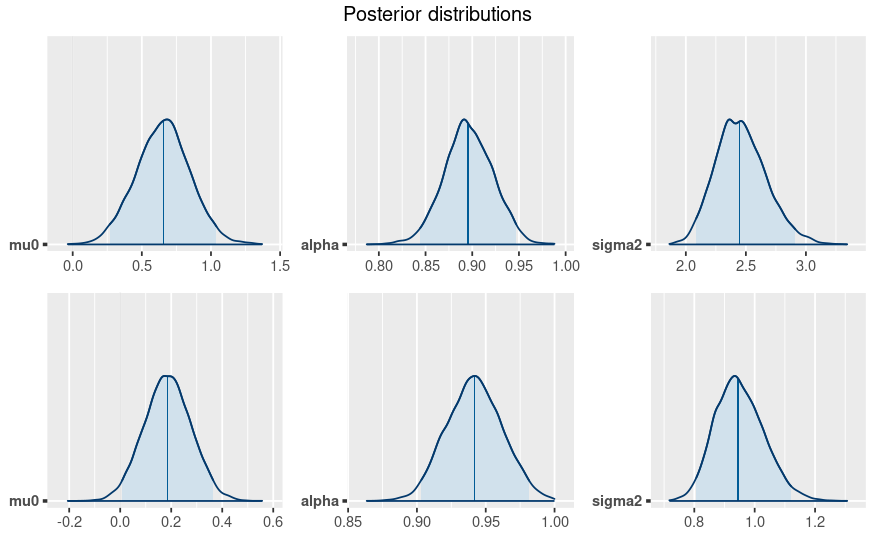
\includegraphics[width=\textwidth]{../Images/2-AR/posteriors.png}
    \caption{The image displays the posterior distributions of the parameters for the AR(1) model. The top line corresponds to the model used for GDP, while the bottom line corresponds to the model used for inflation.}
    \label{fig:AR_posteriors}
\end{figure} \\
Once we assested the validity of the results, we plotted the in-sample and out-of-sample prediction with credible intervals and we compared it with the true data: \\
\begin{figure}[H]
    \centering
    \begin{minipage}[H]{0.7\textwidth}
        \centering
        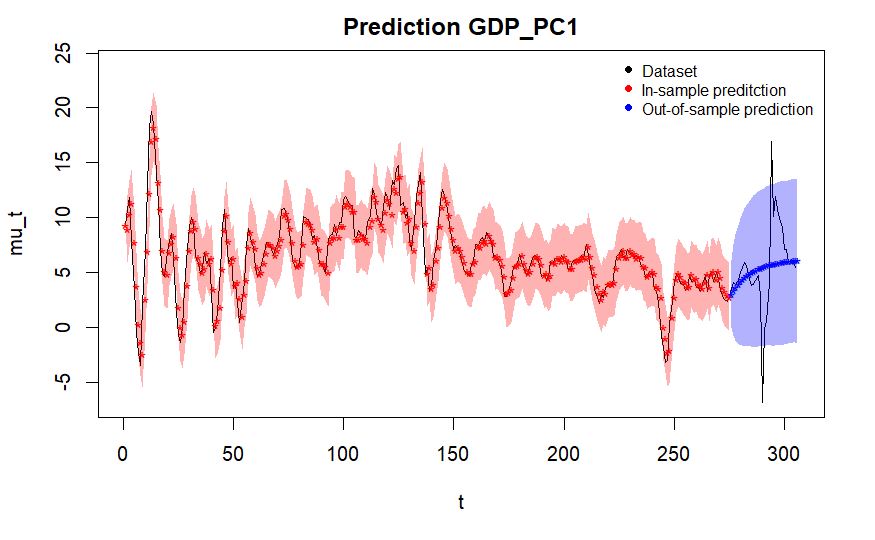
\includegraphics[width=\textwidth]{../Images/2-AR/gdp_prediction.png}
        \label{fig:first}
    \end{minipage}
    \begin{minipage}[H]{0.7\textwidth}
        \centering
        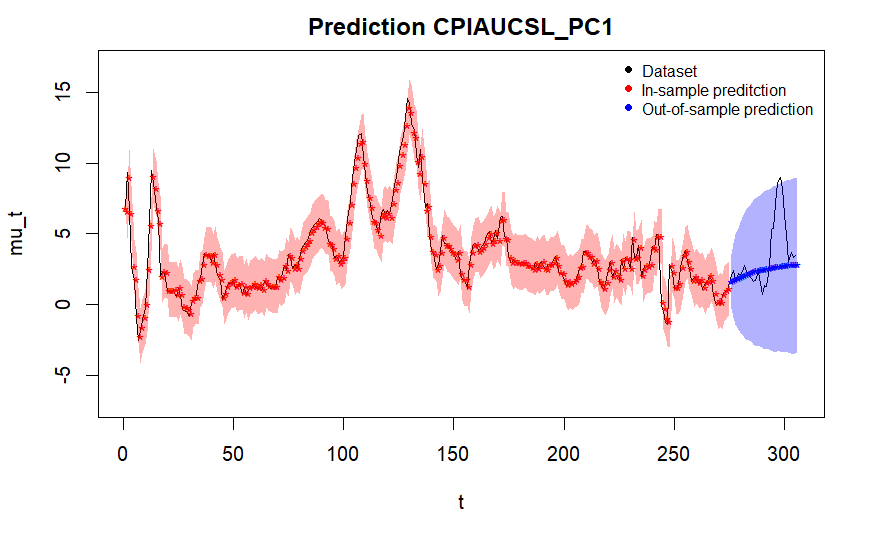
\includegraphics[width=\textwidth]{../Images/2-AR/infl_prediction.png}
        \label{fig:second}
    \end{minipage}
    \caption{In-sample and out-of-sample predictions}
    \label{fig:combined}
\end{figure} \\

We concluded by comparing the model's in-sample predictions and the posterior distributions of its parameters with those obtained from the AR model using the ARIMA function. The detailed comparison results are provided in the Appendix. It was found that there is no significant difference between them. 